\documentclass[10pt]{article}
\usepackage[utf8]{inputenc}
\usepackage[T1]{fontenc}
\usepackage[margin=2.5cm]{geometry}
\usepackage{graphicx}
\usepackage{hyperref}
\usepackage{caption}
\usepackage{setspace}

\doublespacing

\graphicspath{{../figures/}{../../../analysis/results/phase2/}{../../../analysis/results/phase3/}}

\title{\textbf{Supplementary Information}\\[0.5em]
\large Mechanistic Interpretability of Plant Genomic Foundation Models:\\
Dissecting How Transformers Process Plant DNA}

\author{Ihor Kendiukhov}
\date{}

\begin{document}
\maketitle

\section*{Supplementary Figures}

\begin{figure}[h!]
    \centering
    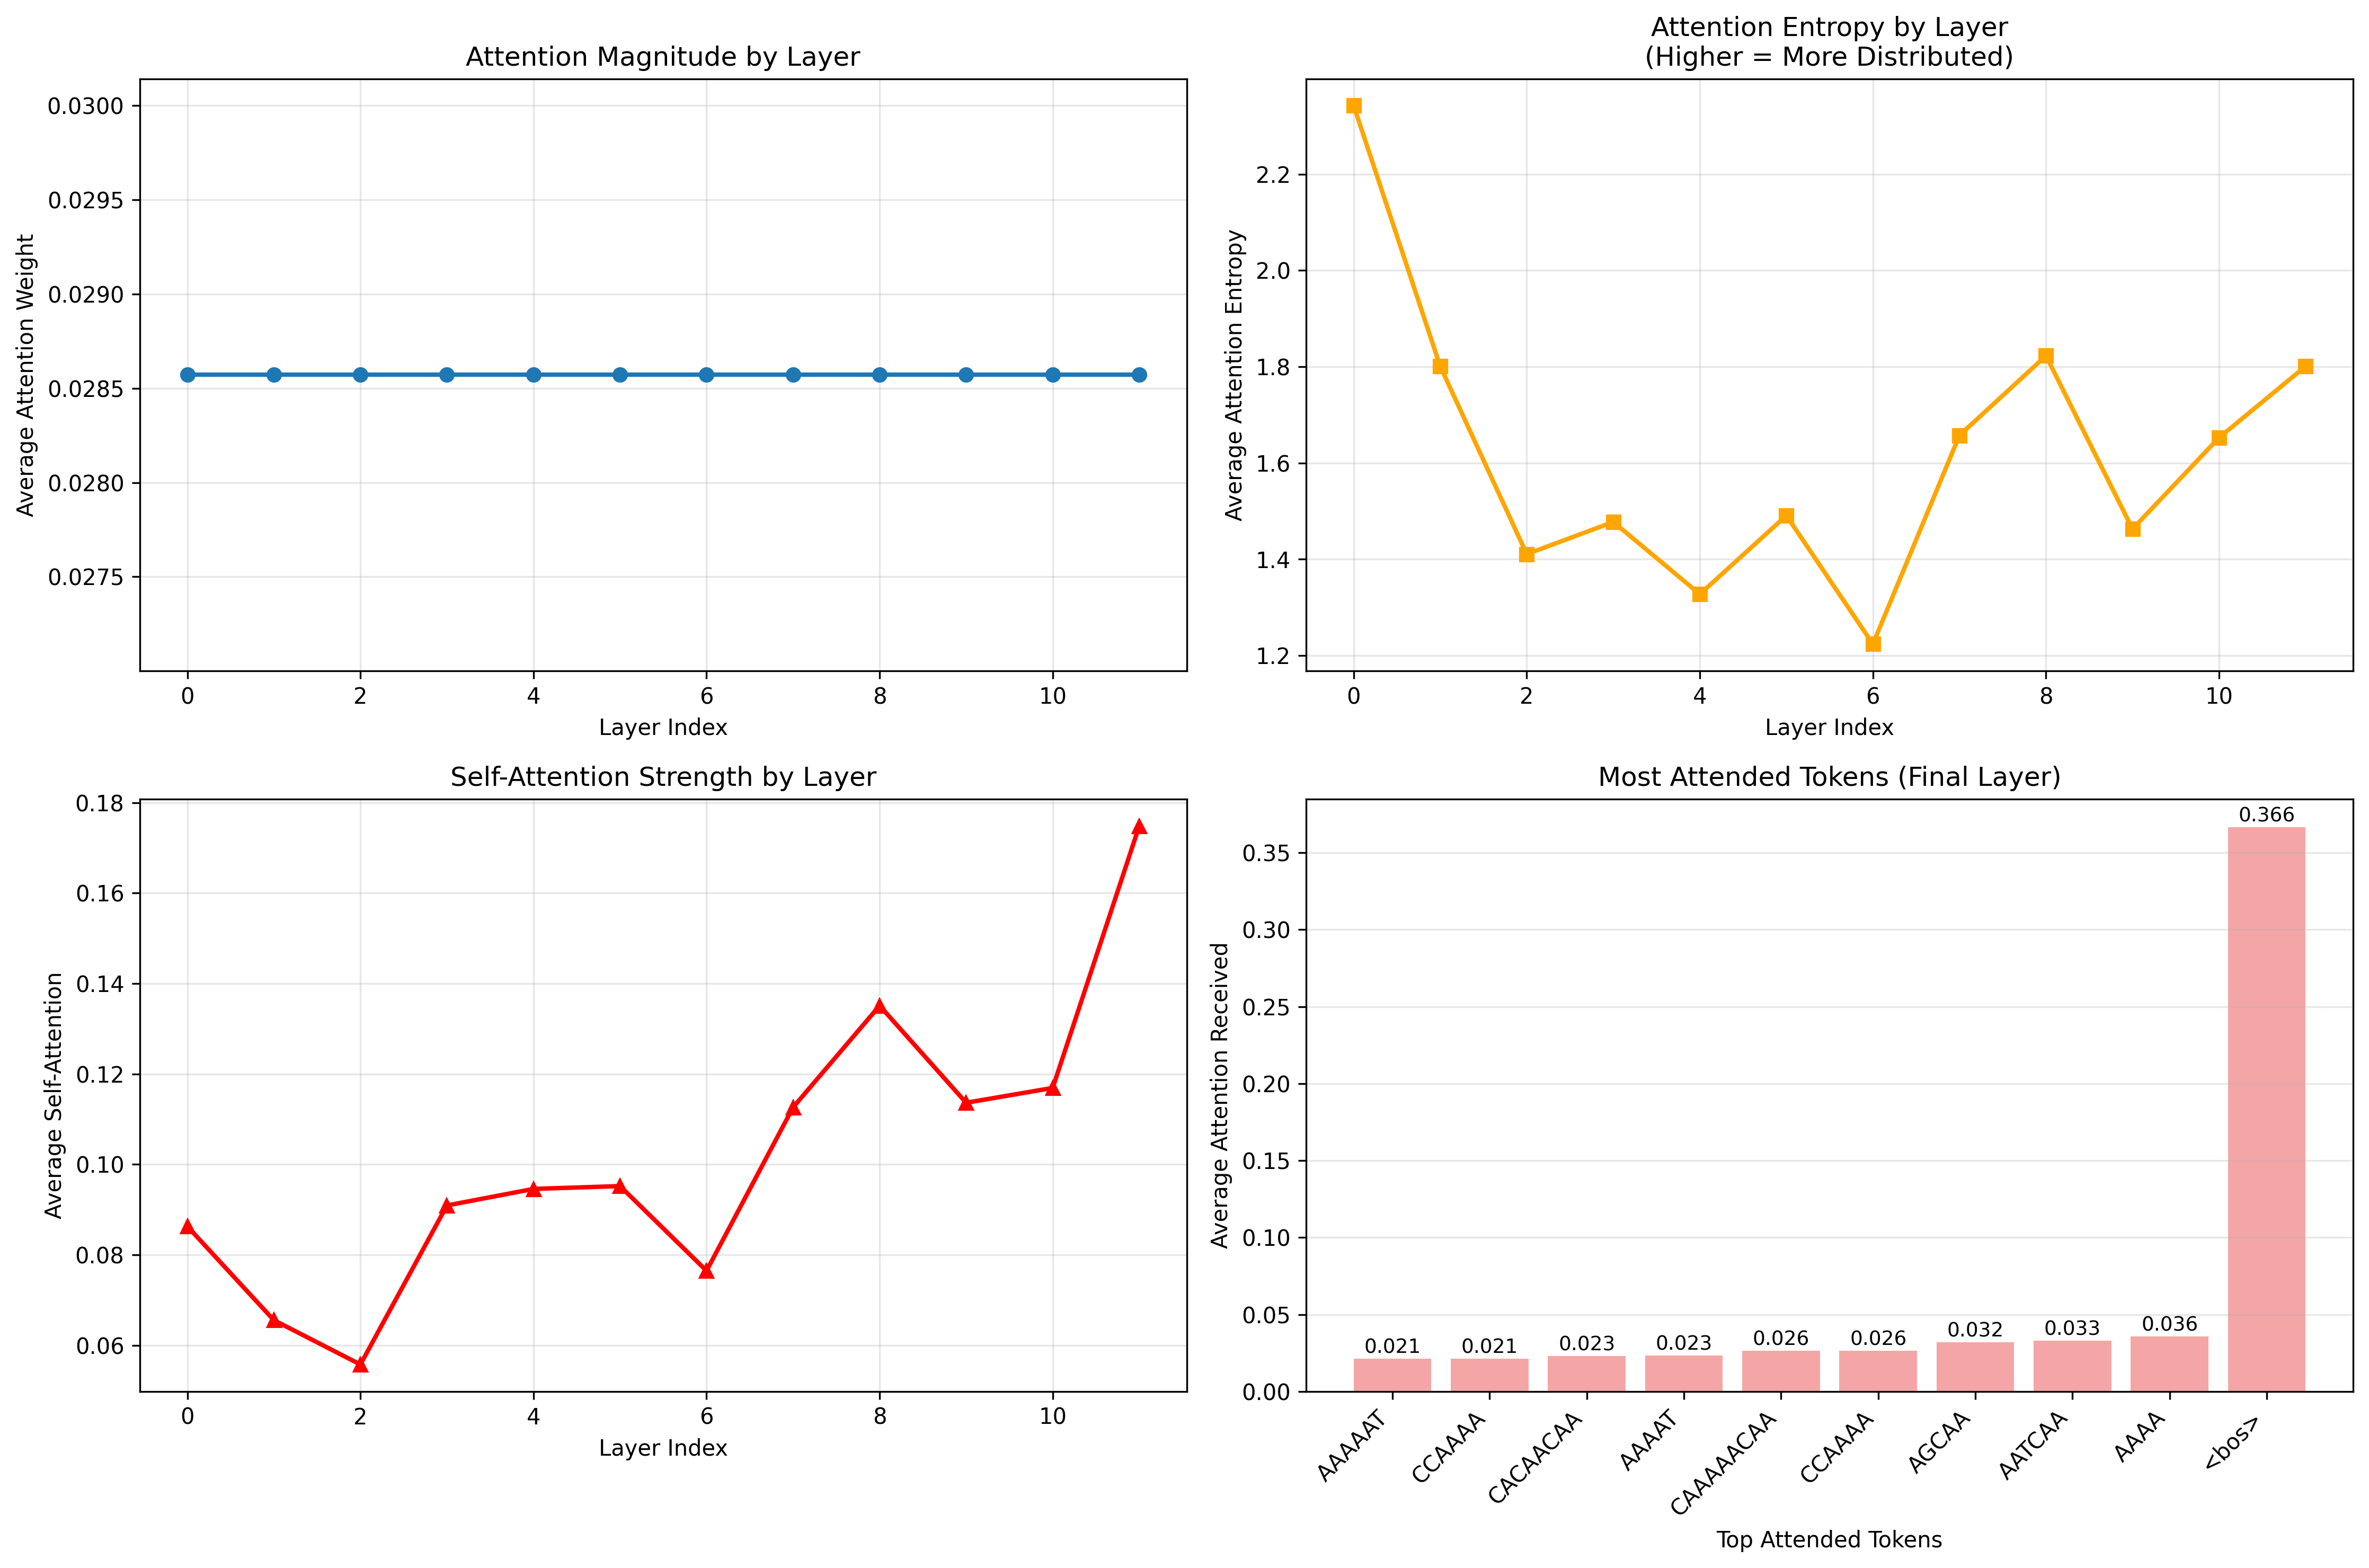
\includegraphics[width=0.8\textwidth]{attention_statistics.png}
    \caption{\textbf{Supplementary Figure S1.} Attention weight statistics across all 144 attention heads in Plant-DnaGemma, showing the distribution of mean attention weights, entropy, and maximum attention values per head.}
\end{figure}

\begin{figure}[h!]
    \centering
    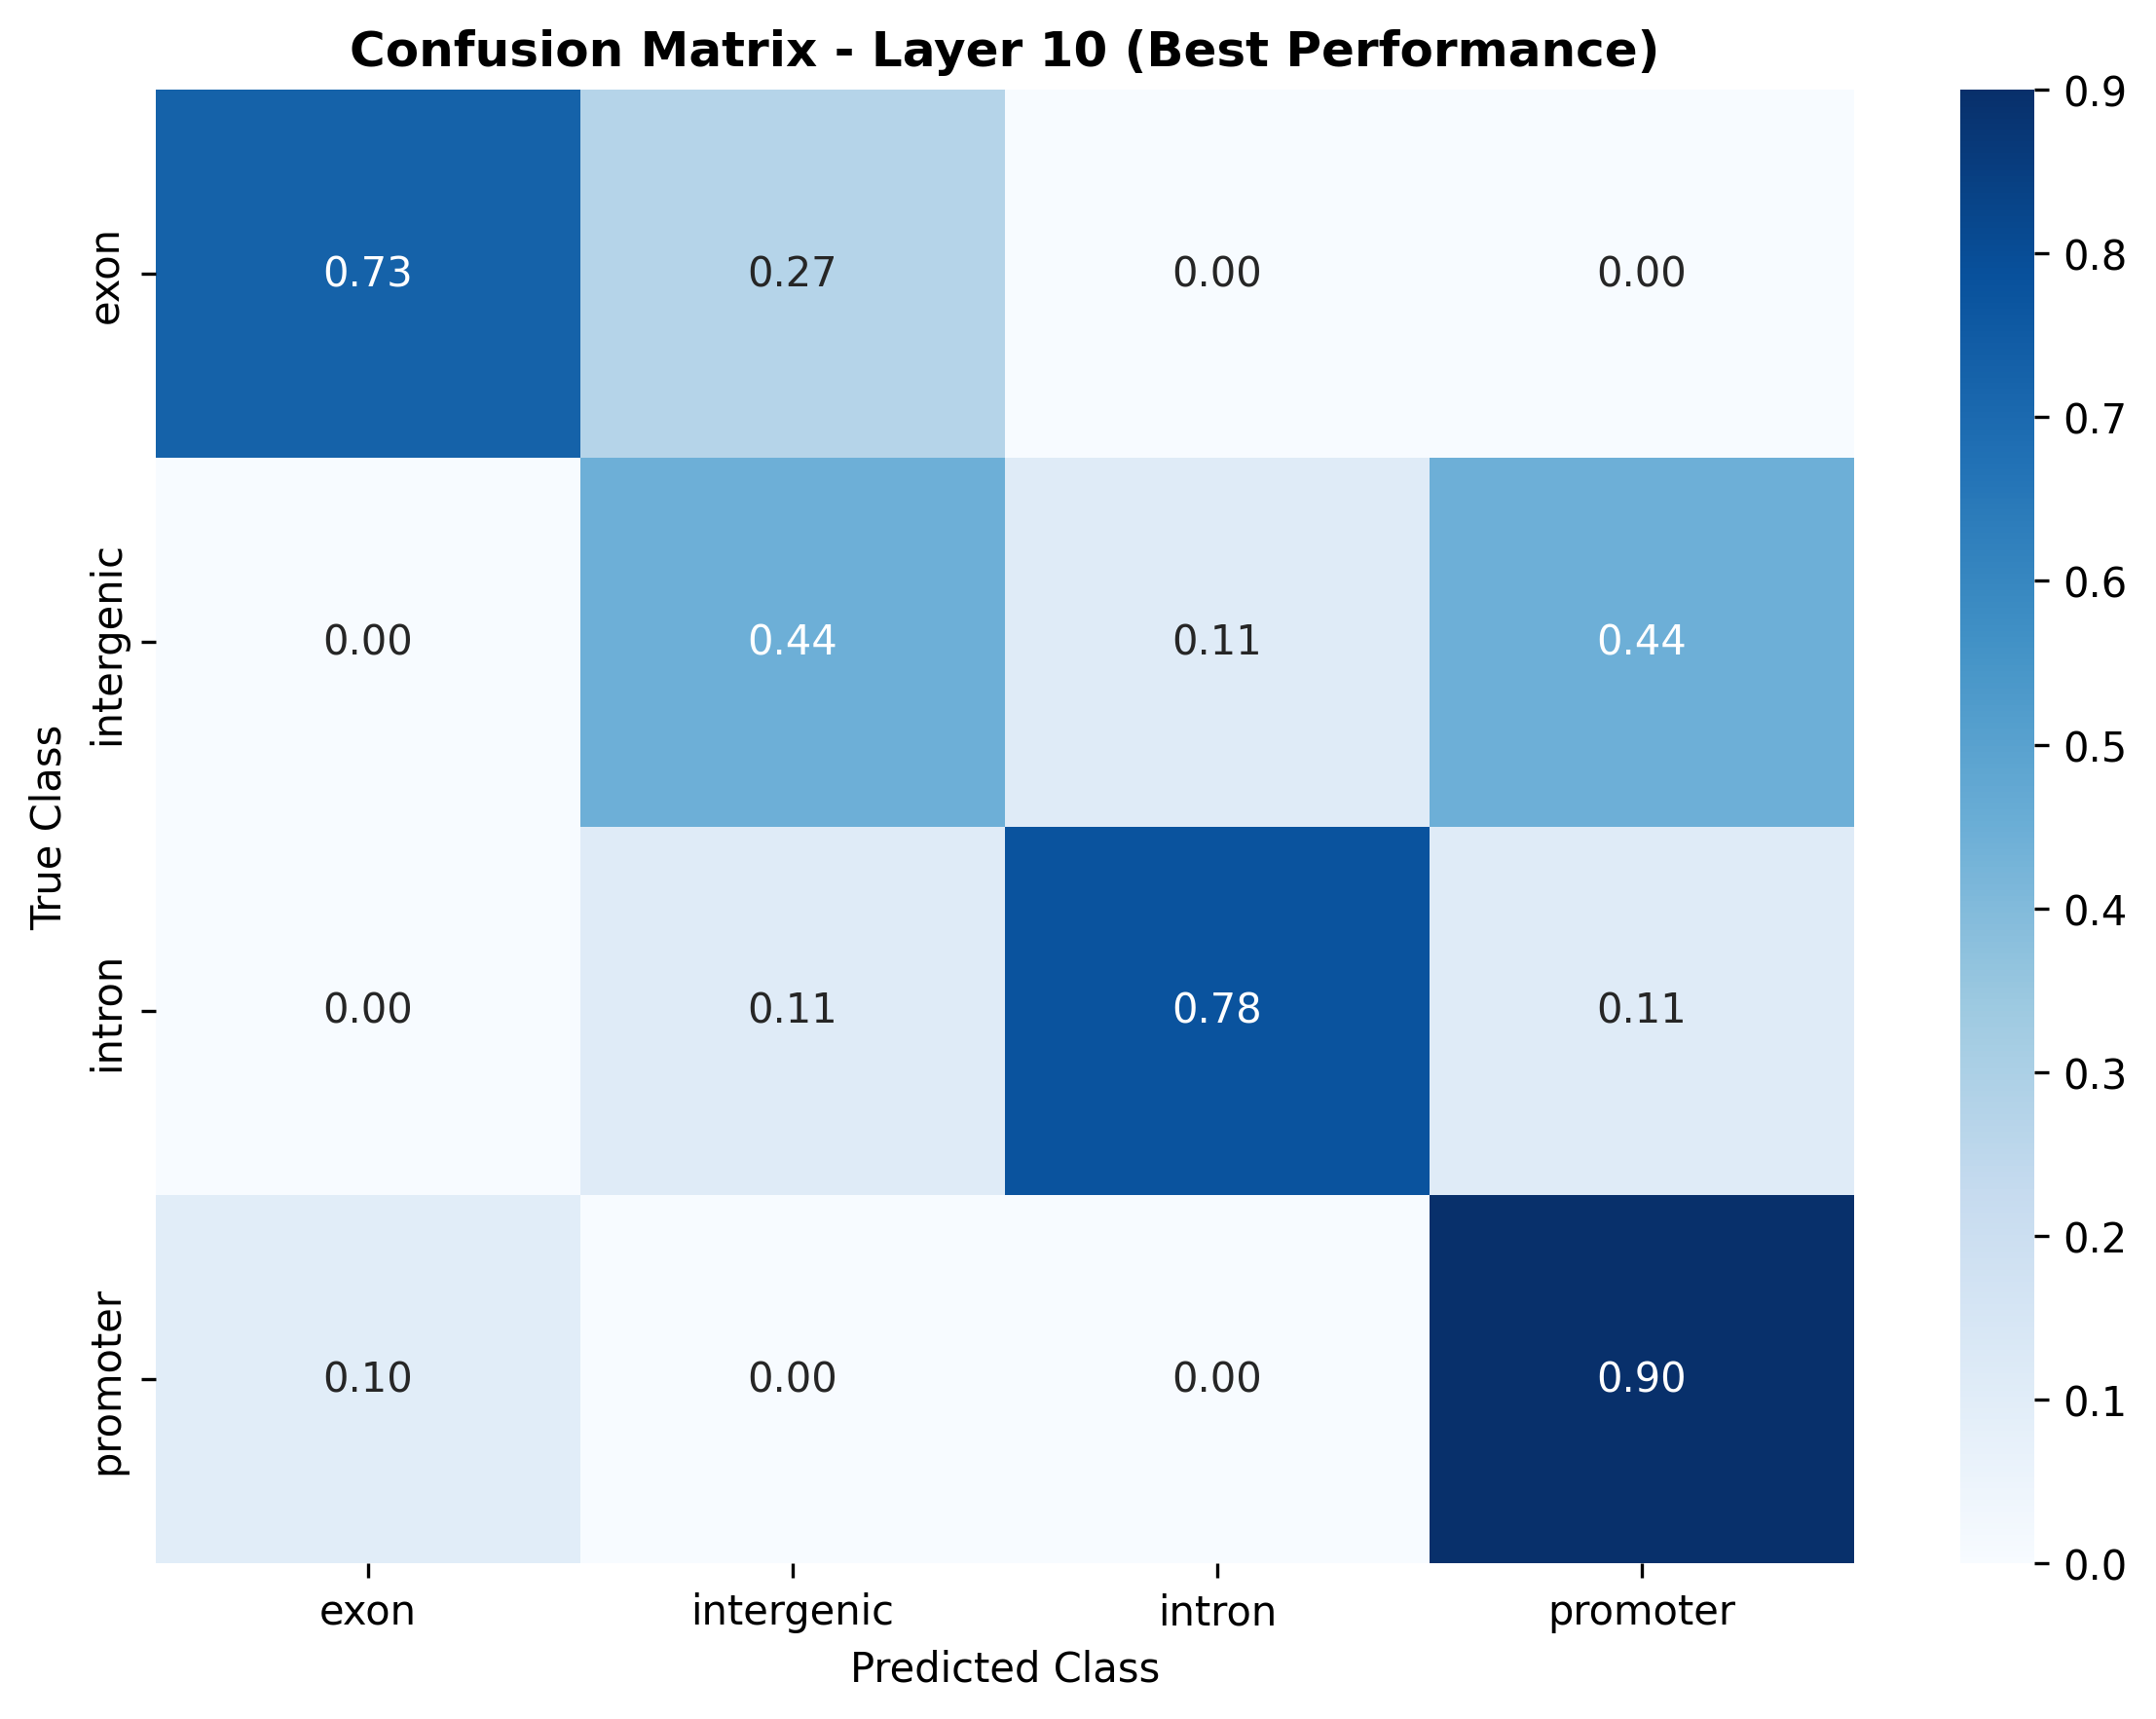
\includegraphics[width=0.7\textwidth]{confusion_matrix_best_layer.png}
    \caption{\textbf{Supplementary Figure S2.} Confusion matrix for the linear probing classifier at layer 10 (best-performing layer), showing classification patterns across the four genomic sequence types.}
\end{figure}

\begin{figure}[h!]
    \centering
    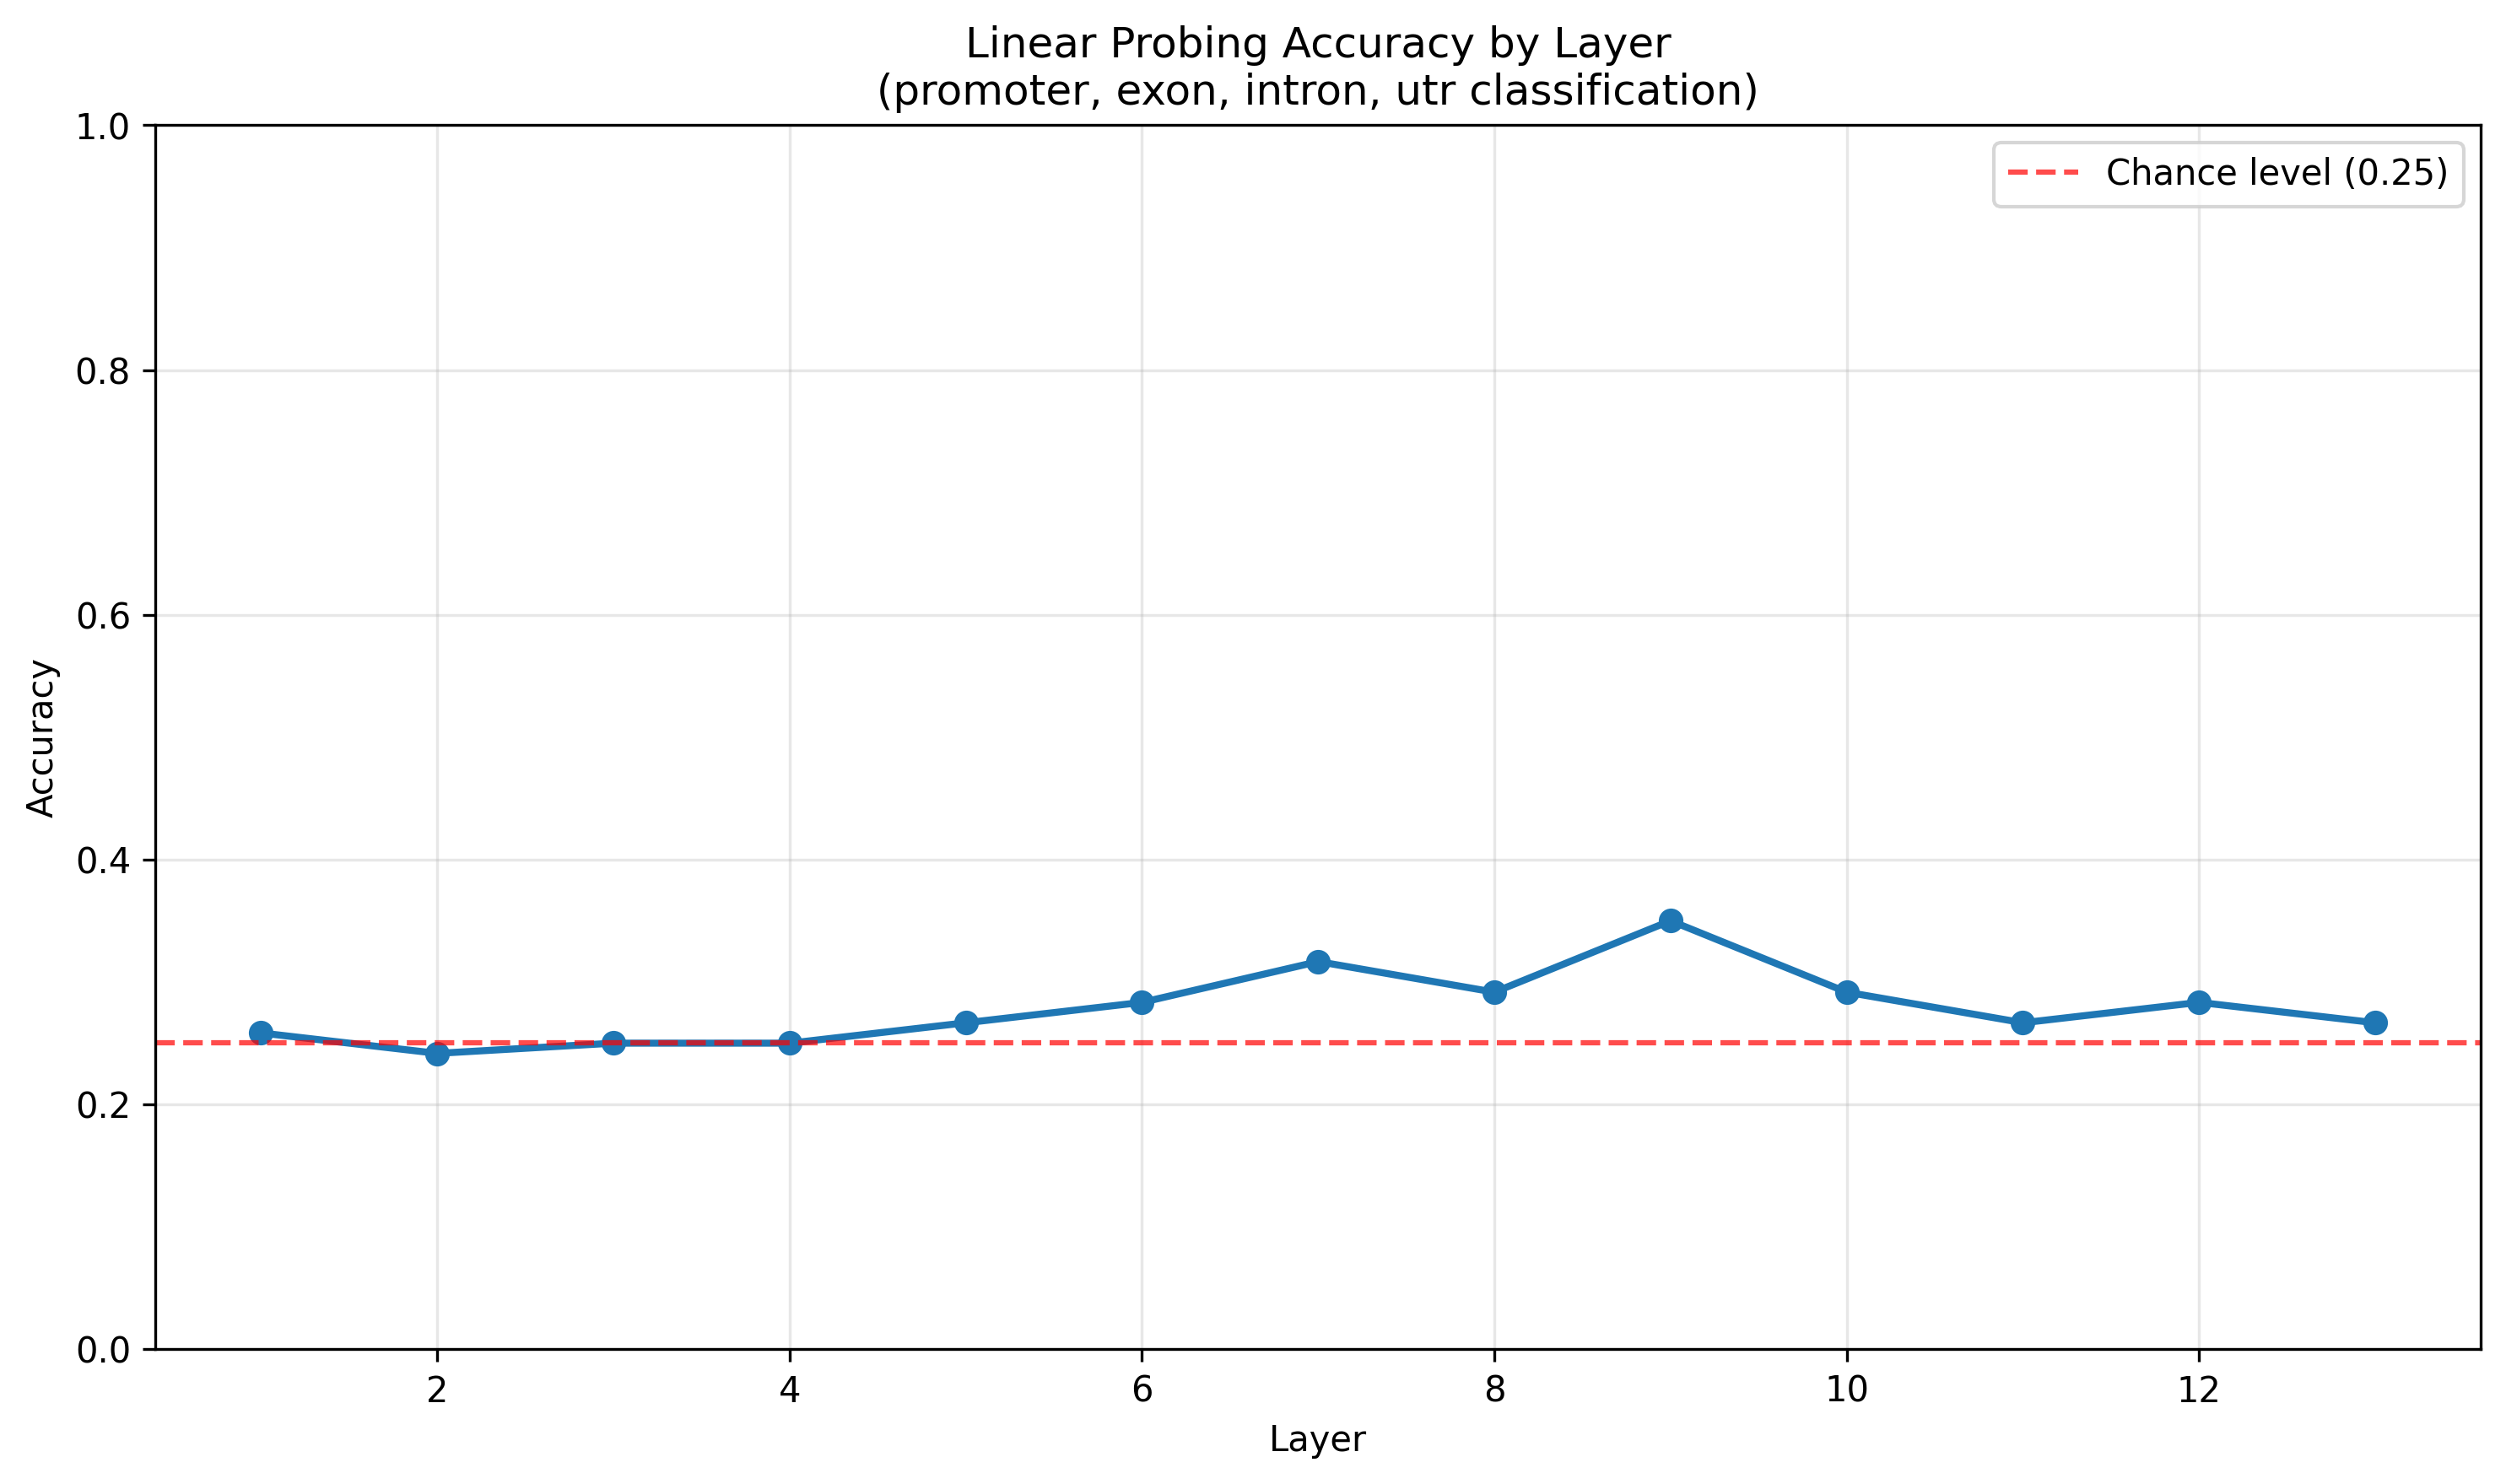
\includegraphics[width=0.7\textwidth]{probing_accuracy_by_layer.png}
    \caption{\textbf{Supplementary Figure S3.} Probing accuracy plotted by layer, showing the progression of classification performance from the embedding layer through all 12 transformer layers.}
\end{figure}

\end{document}
